
%% bare_conf.tex
%% V1.4b
%% 2015/08/26
%% by Michael Shell
%% See:
%% http://www.michaelshell.org/
%% for current contact information.
%%
%% This is a skeleton file demonstrating the use of IEEEtran.cls
%% (requires IEEEtran.cls version 1.8b or later) with an IEEE
%% conference paper.
%%
%% Support sites:
%% http://www.michaelshell.org/tex/ieeetran/
%% http://www.ctan.org/pkg/ieeetran
%% and
%% http://www.ieee.org/

%%*************************************************************************
%% Legal Notice:
%% This code is offered as-is without any warranty either expressed or
%% implied; without even the implied warranty of MERCHANTABILITY or
%% FITNESS FOR A PARTICULAR PURPOSE! 
%% User assumes all risk.
%% In no event shall the IEEE or any contributor to this code be liable for
%% any damages or losses, including, but not limited to, incidental,
%% consequential, or any other damages, resulting from the use or misuse
%% of any information contained here.
%%
%% All comments are the opinions of their respective authors and are not
%% necessarily endorsed by the IEEE.
%%
%% This work is distributed under the LaTeX Project Public License (LPPL)
%% ( http://www.latex-project.org/ ) version 1.3, and may be freely used,
%% distributed and modified. A copy of the LPPL, version 1.3, is included
%% in the base LaTeX documentation of all distributions of LaTeX released
%% 2003/12/01 or later.
%% Retain all contribution notices and credits.
%% ** Modified files should be clearly indicated as such, including  **
%% ** renaming them and changing author support contact information. **
%%*************************************************************************


% *** Authors should verify (and, if needed, correct) their LaTeX system  ***
% *** with the testflow diagnostic prior to trusting their LaTeX platform ***
% *** with production work. The IEEE's font choices and paper sizes can   ***
% *** trigger bugs that do not appear when using other class files.       ***                          ***
% The testflow support page is at:
% http://www.michaelshell.org/tex/testflow/



\documentclass[conference]{IEEEtran}
% Some Computer Society conferences also require the compsoc mode option,
% but others use the standard conference format.
%
% If IEEEtran.cls has not been installed into the LaTeX system files,
% manually specify the path to it like:
% \documentclass[conference]{../sty/IEEEtran}





% Some very useful LaTeX packages include:
% (uncomment the ones you want to load)


% *** MISC UTILITY PACKAGES ***
%
%\usepackage{ifpdf}
% Heiko Oberdiek's ifpdf.sty is very useful if you need conditional
% compilation based on whether the output is pdf or dvi.
% usage:
% \ifpdf
%   % pdf code
% \else
%   % dvi code
% \fi
% The latest version of ifpdf.sty can be obtained from:
% http://www.ctan.org/pkg/ifpdf
% Also, note that IEEEtran.cls V1.7 and later provides a builtin
% \ifCLASSINFOpdf conditional that works the same way.
% When switching from latex to pdflatex and vice-versa, the compiler may
% have to be run twice to clear warning/error messages.






% *** CITATION PACKAGES ***
%
%\usepackage{cite}
% cite.sty was written by Donald Arseneau
% V1.6 and later of IEEEtran pre-defines the format of the cite.sty package
% \cite{} output to follow that of the IEEE. Loading the cite package will
% result in citation numbers being automatically sorted and properly
% "compressed/ranged". e.g., [1], [9], [2], [7], [5], [6] without using
% cite.sty will become [1], [2], [5]--[7], [9] using cite.sty. cite.sty's
% \cite will automatically add leading space, if needed. Use cite.sty's
% noadjust option (cite.sty V3.8 and later) if you want to turn this off
% such as if a citation ever needs to be enclosed in parenthesis.
% cite.sty is already installed on most LaTeX systems. Be sure and use
% version 5.0 (2009-03-20) and later if using hyperref.sty.
% The latest version can be obtained at:
% http://www.ctan.org/pkg/cite
% The documentation is contained in the cite.sty file itself.






% *** GRAPHICS RELATED PACKAGES ***
%
\ifCLASSINFOpdf
  % \usepackage[pdftex]{graphicx}
  % declare the path(s) where your graphic files are
  % \graphicspath{{../pdf/}{../jpeg/}}
  % and their extensions so you won't have to specify these with
  % every instance of \includegraphics
  % \DeclareGraphicsExtensions{.pdf,.jpeg,.png}
\else
  % or other class option (dvipsone, dvipdf, if not using dvips). graphicx
  % will default to the driver specified in the system graphics.cfg if no
  % driver is specified.
  % \usepackage[dvips]{graphicx}
  % declare the path(s) where your graphic files are
  % \graphicspath{{../eps/}}
  % and their extensions so you won't have to specify these with
  % every instance of \includegraphics
  % \DeclareGraphicsExtensions{.eps}
\fi
% graphicx was written by David Carlisle and Sebastian Rahtz. It is
% required if you want graphics, photos, etc. graphicx.sty is already
% installed on most LaTeX systems. The latest version and documentation
% can be obtained at: 
% http://www.ctan.org/pkg/graphicx
% Another good source of documentation is "Using Imported Graphics in
% LaTeX2e" by Keith Reckdahl which can be found at:
% http://www.ctan.org/pkg/epslatex
%
% latex, and pdflatex in dvi mode, support graphics in encapsulated
% postscript (.eps) format. pdflatex in pdf mode supports graphics
% in .pdf, .jpeg, .png and .mps (metapost) formats. Users should ensure
% that all non-photo figures use a vector format (.eps, .pdf, .mps) and
% not a bitmapped formats (.jpeg, .png). The IEEE frowns on bitmapped formats
% which can result in "jaggedy"/blurry rendering of lines and letters as
% well as large increases in file sizes.
%
% You can find documentation about the pdfTeX application at:
% http://www.tug.org/applications/pdftex





% *** MATH PACKAGES ***
%
%\usepackage{amsmath}
% A popular package from the American Mathematical Society that provides
% many useful and powerful commands for dealing with mathematics.
%
% Note that the amsmath package sets \interdisplaylinepenalty to 10000
% thus preventing page breaks from occurring within multiline equations. Use:
%\interdisplaylinepenalty=2500
% after loading amsmath to restore such page breaks as IEEEtran.cls normally
% does. amsmath.sty is already installed on most LaTeX systems. The latest
% version and documentation can be obtained at:
% http://www.ctan.org/pkg/amsmath





% *** SPECIALIZED LIST PACKAGES ***
%
%\usepackage{algorithmic}
% algorithmic.sty was written by Peter Williams and Rogerio Brito.
% This package provides an algorithmic environment fo describing algorithms.
% You can use the algorithmic environment in-text or within a figure
% environment to provide for a floating algorithm. Do NOT use the algorithm
% floating environment provided by algorithm.sty (by the same authors) or
% algorithm2e.sty (by Christophe Fiorio) as the IEEE does not use dedicated
% algorithm float types and packages that provide these will not provide
% correct IEEE style captions. The latest version and documentation of
% algorithmic.sty can be obtained at:
% http://www.ctan.org/pkg/algorithms
% Also of interest may be the (relatively newer and more customizable)
% algorithmicx.sty package by Szasz Janos:
% http://www.ctan.org/pkg/algorithmicx




% *** ALIGNMENT PACKAGES ***
%
%\usepackage{array}
% Frank Mittelbach's and David Carlisle's array.sty patches and improves
% the standard LaTeX2e array and tabular environments to provide better
% appearance and additional user controls. As the default LaTeX2e table
% generation code is lacking to the point of almost being broken with
% respect to the quality of the end results, all users are strongly
% advised to use an enhanced (at the very least that provided by array.sty)
% set of table tools. array.sty is already installed on most systems. The
% latest version and documentation can be obtained at:
% http://www.ctan.org/pkg/array


% IEEEtran contains the IEEEeqnarray family of commands that can be used to
% generate multiline equations as well as matrices, tables, etc., of high
% quality.




% *** SUBFIGURE PACKAGES ***
%\ifCLASSOPTIONcompsoc
%  \usepackage[caption=false,font=normalsize,labelfont=sf,textfont=sf]{subfig}
%\else
%  \usepackage[caption=false,font=footnotesize]{subfig}
%\fi
% subfig.sty, written by Steven Douglas Cochran, is the modern replacement
% for subfigure.sty, the latter of which is no longer maintained and is
% incompatible with some LaTeX packages including fixltx2e. However,
% subfig.sty requires and automatically loads Axel Sommerfeldt's caption.sty
% which will override IEEEtran.cls' handling of captions and this will result
% in non-IEEE style figure/table captions. To prevent this problem, be sure
% and invoke subfig.sty's "caption=false" package option (available since
% subfig.sty version 1.3, 2005/06/28) as this is will preserve IEEEtran.cls
% handling of captions.
% Note that the Computer Society format requires a larger sans serif font
% than the serif footnote size font used in traditional IEEE formatting
% and thus the need to invoke different subfig.sty package options depending
% on whether compsoc mode has been enabled.
%
% The latest version and documentation of subfig.sty can be obtained at:
% http://www.ctan.org/pkg/subfig




% *** FLOAT PACKAGES ***
%
%\usepackage{fixltx2e}
% fixltx2e, the successor to the earlier fix2col.sty, was written by
% Frank Mittelbach and David Carlisle. This package corrects a few problems
% in the LaTeX2e kernel, the most notable of which is that in current
% LaTeX2e releases, the ordering of single and double column floats is not
% guaranteed to be preserved. Thus, an unpatched LaTeX2e can allow a
% single column figure to be placed prior to an earlier double column
% figure.
% Be aware that LaTeX2e kernels dated 2015 and later have fixltx2e.sty's
% corrections already built into the system in which case a warning will
% be issued if an attempt is made to load fixltx2e.sty as it is no longer
% needed.
% The latest version and documentation can be found at:
% http://www.ctan.org/pkg/fixltx2e


%\usepackage{stfloats}
% stfloats.sty was written by Sigitas Tolusis. This package gives LaTeX2e
% the ability to do double column floats at the bottom of the page as well
% as the top. (e.g., "\begin{figure*}[!b]" is not normally possible in
% LaTeX2e). It also provides a command:
%\fnbelowfloat
% to enable the placement of footnotes below bottom floats (the standard
% LaTeX2e kernel puts them above bottom floats). This is an invasive package
% which rewrites many portions of the LaTeX2e float routines. It may not work
% with other packages that modify the LaTeX2e float routines. The latest
% version and documentation can be obtained at:
% http://www.ctan.org/pkg/stfloats
% Do not use the stfloats baselinefloat ability as the IEEE does not allow
% \baselineskip to stretch. Authors submitting work to the IEEE should note
% that the IEEE rarely uses double column equations and that authors should try
% to avoid such use. Do not be tempted to use the cuted.sty or midfloat.sty
% packages (also by Sigitas Tolusis) as the IEEE does not format its papers in
% such ways.
% Do not attempt to use stfloats with fixltx2e as they are incompatible.
% Instead, use Morten Hogholm'a dblfloatfix which combines the features
% of both fixltx2e and stfloats:
%
% \usepackage{dblfloatfix}
% The latest version can be found at:
% http://www.ctan.org/pkg/dblfloatfix




% *** PDF, URL AND HYPERLINK PACKAGES ***
%
%\usepackage{url}
% url.sty was written by Donald Arseneau. It provides better support for
% handling and breaking URLs. url.sty is already installed on most LaTeX
% systems. The latest version and documentation can be obtained at:
% http://www.ctan.org/pkg/url
% Basically, \url{my_url_here}.




% *** Do not adjust lengths that control margins, column widths, etc. ***
% *** Do not use packages that alter fonts (such as pslatex).         ***
% There should be no need to do such things with IEEEtran.cls V1.6 and later.
% (Unless specifically asked to do so by the journal or conference you plan
% to submit to, of course. )

\usepackage{tabularx}
\usepackage{lipsum}
\usepackage{blindtext}
\usepackage{graphicx}

\newcolumntype{K}[1]{>{\centering\arraybackslash}p{#1}}



% correct bad hyphenation here
\hyphenation{op-tical net-works semi-conduc-tor}


\begin{document}
%
% paper title
% Titles are generally capitalized except for words such as a, an, and, as,
% at, but, by, for, in, nor, of, on, or, the, to and up, which are usually
% not capitalized unless they are the first or last word of the title.
% Linebreaks \\ can be used within to get better formatting as desired.
% Do not put math or special symbols in the title.
\title{Cyber vs Regular: A Comparison of Consumer Fraud in The United States}


% author names and affiliations
% use a multiple column layout for up to three different
% affiliations


%\author{\IEEEauthorblockN{Mohammad Taha Khan and Chris Kanich}
%\IEEEauthorblockA{Department of Computer Science, University of Illinois at Chicago\\taha@cs.uic.edu, ckanich@uic.edu}}

% conference papers do not typically use \thanks and this command
% is locked out in conference mode. If really needed, such as for
% the acknowledgment of grants, issue a \IEEEoverridecommandlockouts
% after \documentclass

% for over three affiliations, or if they all won't fit within the width
% of the page, use this alternative format:
% 
%\author{\IEEEauthorblockN{Michael Shell\IEEEauthorrefmark{1},
%Homer Simpson\IEEEauthorrefmark{2},
%James Kirk\IEEEauthorrefmark{3}, 
%Montgomery Scott\IEEEauthorrefmark{3} and
%Eldon Tyrell\IEEEauthorrefmark{4}}
%\IEEEauthorblockA{\IEEEauthorrefmark{1}School of Electrical and Computer Engineering\\
%Georgia Institute of Technology,
%Atlanta, Georgia 30332--0250\\ Email: see http://www.michaelshell.org/contact.html}
%\IEEEauthorblockA{\IEEEauthorrefmark{2}Twentieth Century Fox, Springfield, USA\\
%Email: homer@thesimpsons.com}
%\IEEEauthorblockA{\IEEEauthorrefmark{3}Starfleet Academy, San Francisco, California 96678-2391\\
%Telephone: (800) 555--1212, Fax: (888) 555--1212}
%\IEEEauthorblockA{\IEEEauthorrefmark{4}Tyrell Inc., 123 Replicant Street, Los Angeles, California 90210--4321}}




% use for special paper notices
%\IEEEspecialpapernotice{(Invited Paper)}




% make the title area
\maketitle

% As a general rule, do not put math, special symbols or citations
% in the abstract
\begin{abstract}
\lipsum[2-3]
\end{abstract}

% no keywords




% For peer review papers, you can put extra information on the cover
% page as needed:
% \ifCLASSOPTIONpeerreview
% \begin{center} \bfseries EDICS Category: 3-BBND \end{center}
% \fi
%
% For peerreview papers, this IEEEtran command inserts a page break and
% creates the second title. It will be ignored for other modes.
\IEEEpeerreviewmaketitle


\section{Introduction}
the main contributions:
Understanding the differences in the  nature of cyber and regular frauds in the United States.
Exploring if certain demographics are more succeptible to cybercrime
Suggesting improvements that might be the right way to create more awareness annd campaings.


Fraud and and deceptive practices have been around since the establishment of 


The FTC and the FBI 



\lipsum[2-7]

\section{Related Work}




\begin{table*}[h]
\noindent
\centering
\begin{tabular}{|K{0.18\linewidth}|p{0.72\linewidth}|}
\hline
\multicolumn{1}{|c|}{\bfseries Data Field} & \multicolumn{1}{c|}{\bfseries Field Description}
\\ 
\hline
Agency Name & All the complaint collection agencies associated with the FTC. Some of the prominent  agencies were the FTC online and phone centers, publisher clearing house and the attorney general in specific states.\\
\hline
Zip code Information & The zip code of the victim and the fraudulent entity. This provided us with low level granularity for analysis, however, the latter was only available for a subset of the complaints\\
\hline
Contact Method & The Primary channel method that was used by the fraudulet entity to contact the victim e.g. Internet, phone, mail.\\
\hline
Fraud Description & A description of nature the fraud, and its type e.g. credit  card, fake product, business fraud.\\
\hline
Fraud \&
 Reporting Date & The dates when the fraud initially occurred and the date on which is was reported
\\
\hline
\end{tabular}
\bigskip
\caption{The description of the data fields that were primarily used in the for data calibration and analysis}\label{ftcdata}
\end{table*}




As our work evaluates both cyber as well as regular frauds, we provide related work that encompasses both of these categories. However, we elaborate more on recent research which focuses on cyber frauds
as more individuals are victims of these crimes \cite{ftcfraud} due to the increased Internet usage trends for sensitive activities. Before the Internet became a primary hub of economic and social activity, researchers measured \cite{ukphone} and developed techniques based on statistical models \cite{creditfraud, phoenfraudnn, phonefraudstat} to detect phone and credit card based frauds. In the past few years,  research evaluations have shifted focus towards cyber activity \cite{databreach, playingfield, fraudfinance, cybertrends} due to its high rate and the potential for harm.

Even though, term \emph{"cyber"} is usually associated with Computer Science, due to its recent socio-economic impact, researchers in Economics, Law, and Finance have also explored for solutions to this problem by incorporating methodologies specific to their areas. Ionescu et. al \cite{fraudfinance} characterize the types and sources cyber frauds in global digital networks. The authors link the exponential increase of cyber fraud to increased Internet usage for financial management and transactions, especially in financial markets. They suggest the involvement of all stakeholders and employees through awareness and training for containing and mitigating fraud. Similarly, Howard et. al \cite{cybertrends} study malicious code attacks against financial networks and suggest technical detection and mitigation techniques for financial infrastructure. \cite{playingfield} studies how the cyber criminals have several potential advantages over their opposing law enforcement agencies. They suggest some practical steps to even out the differential gap.


Due to an increase in the overall concern for online fraudulent activity, there has also been state-sponsored research that measures the impact of fraud. Smyth et. al \cite{fraudcanada} measure the extent of cyber fraud in Canada in 2011. Their work indicates that a major chunk of frauds does not get recorded and suggest a need for a sentinel record fraud data, similar to the FTC complaint center in the US.

Another significant area of research focuses on understanding the demographics of fraud victims. A recent FTC Report \cite{ftccomplaints} uses complaint data to quantify complaint rates and across different ethnic and education groups in the US. \cite{consurmeraffairs} also look at how demographics effect the likelyhood of an individual to complain about fraud. Researchers in \cite{databreach} provide a comprehensive survey report that sums the reactions of the victims of an online data breach. They categorize their results in different income, education, age, and ethnic groups. Such research aims to provide organizations with informed insight to better develop policies for consumer rights protection.

In comparison to previous research which individually look at either cyber of regular fraud, our work provides a unique angle of evaluation. We provide a comparison for both types of frauds and describe certain complaint charectaristics and demographic trends which more prevalent in each specific category.


\section{Data and Callibration}

In this section we explain the charectarisitcs of our datasets and the sources they were obtained from. We also provide insight into the essential data processing and callibration methodology that we incorporate to classify and filter the data for a fair evaluation of our questions.

\subsection{Data Description}

\subsubsection{FTC Complaint Dataset}

The primary dataset that we use for our evlauation is a corpus of the complaint logs filed at different collecitons agencies for the FTC during the years 2013-2014. The Dataset comprises of a total of 865K complaints aggregated for cyber as well as regular fraud instances during the time period. Table \ref{ftcdata} shows the fields of the original dataset along with their description summary. For the purposes of brevity, we only include the fields that were used in our analysis.
\\
\subsubsection{US Census Datasets}
Zip code information in our complaint dataset allows us to perform demographic analysis of the frauds. We obtain the demographic information associated with zip codes available at the US Census Bureau website \cite{usbureau}. The specific information that we collect is stated below:

\begin{itemize}
\vspace{8pt}
  \item Population density per zip code
  \item Employment and income data
  \item Age statistics
  \item Race and ethinic information
  \vspace{8pt}
\end{itemize}

As zip codes provide a low level granularity, to aggregate adjacent zip codes we obtain the Zip codes to the Metropolitinan Statistical Area (MSA) mappings from \cite{deptlabor}. MSA are essentially groups of geographically connected zip codes that demonstrate strong social andd economic linkage. While there are more than 40,000 zip codes in the United States there are only 382 distinct MSAs \cite{usbureau}.

\subsection{Calibration Methodology}

\begin{figure}
\centering
  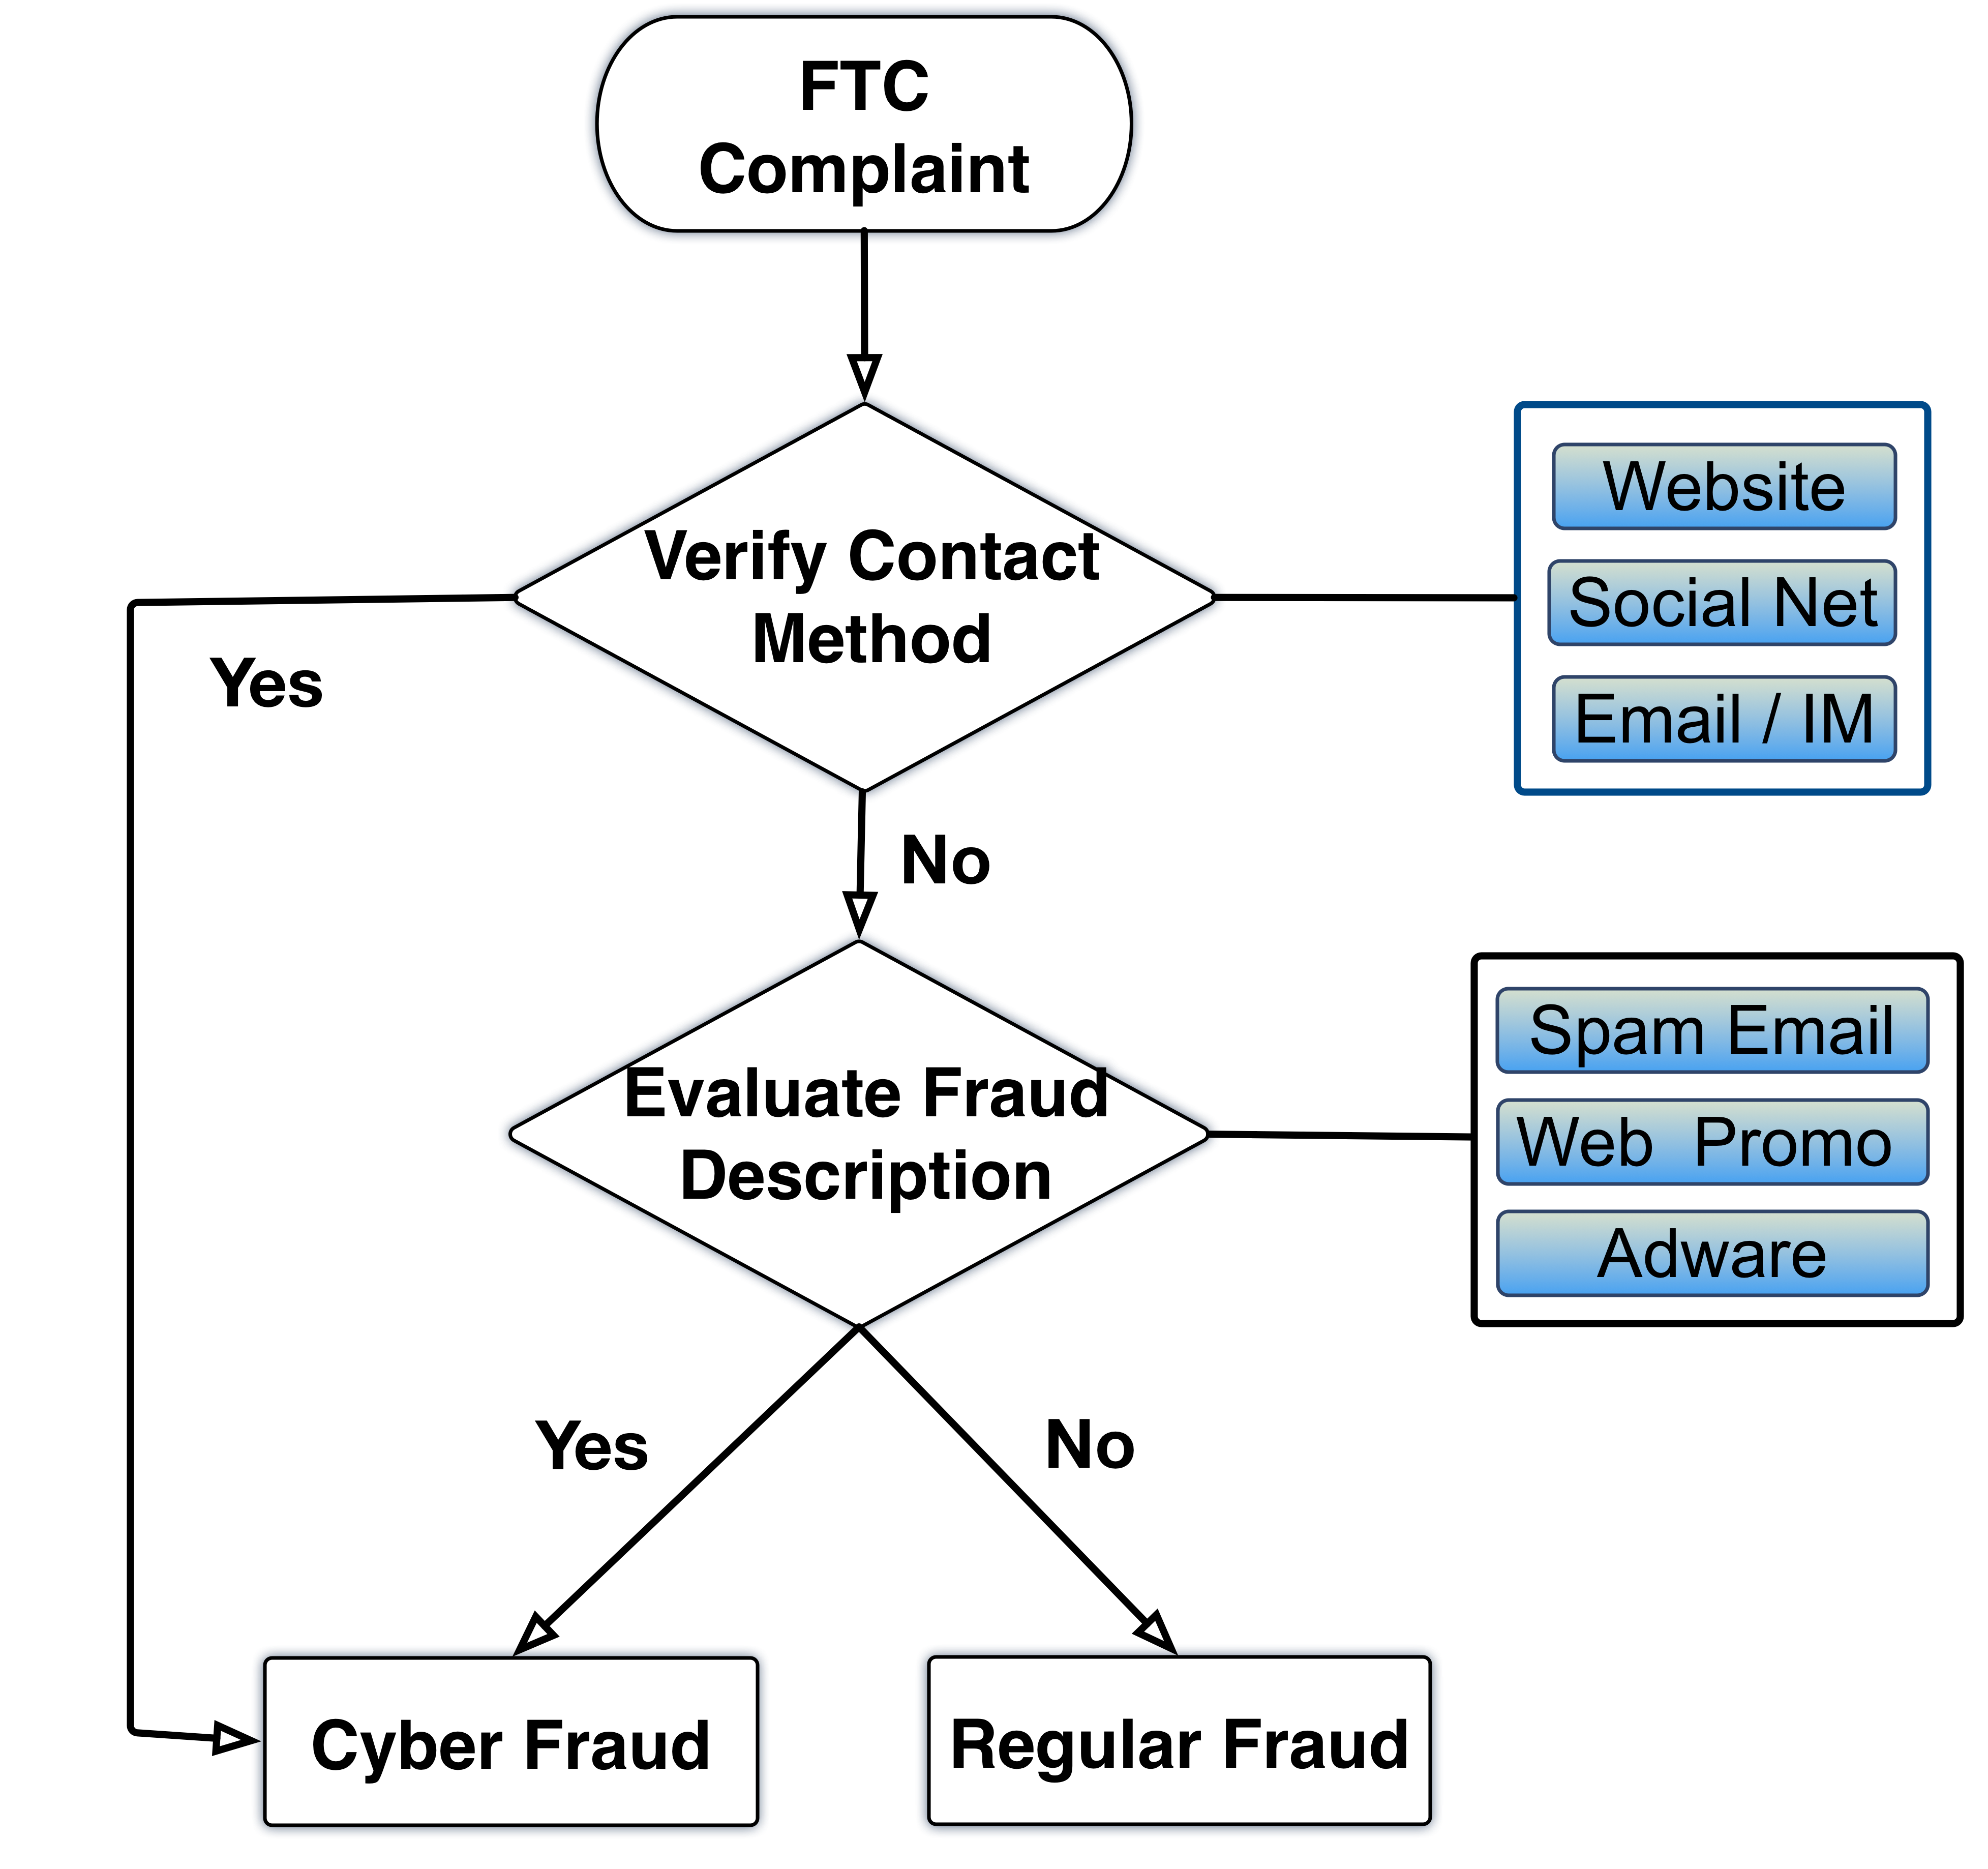
\includegraphics[scale=0.5]{graphics/methodology.png}
  \caption{A boat.}
  \label{classify}
\end{figure}

While information from the US Bureau was standardized and did not require preprocessing, we cater for inconsitencies in the FTC dataset. We realize the the major source of irregularity as a results of its collection ftom various complaint collection agencies furthered by the lack of sanity checks in complaint forms or as a cause of human error while infromation entry. The two major forms of inconsitencies that we filter our are irregular zip codes that cannot be associated with a geographic region in the US and complaints that were missing essential information that required them to be tagged as a cyber of regular fraud.

As the FTC dataset was aggregated for all fraud channels a major calibration step we perfrom is to tag each crime complaint as either cyber or regular. An associated challenge for this was our limited view of the fraud description. To perform this calibration we use the \textbf{Contact Method} and \textbf{Fraud Description} fields from Table \ref{ftcdata}. We flag a complaint as cyber if the victims primary contact method was thorugh online media, these are primarily websites, social networks, email and IM. For the remainder of the complaints we look at the description. If the complinat description invovles something associated with Internet, we classify it as a cyber fraud regardless of how the victim was initially approached. Figure \ref{classify} provides an depicticon of our classification methodology. This process  provides us with two distinct categories  and enables a fair comparison of the frauds. 






\section{Evaluation}


\section{Discussion}


\section{Conclusion}
The conclusion goes here.



\section*{Acknowledgment}


The authors would like to thank...






\begin{thebibliography}{1}

\bibitem{IEEEhowto:kopka}
H.~Kopka and P.~W. Daly, \emph{A Guide to \LaTeX}, 3rd~ed.\hskip 1em plus
  0.5em minus 0.4em\relax Harlow, England: Addison-Wesley, 1999.
  
\bibitem{affiliate}
pete snyder affiliate fraud

\bibitem{fraudfinance}
cyberfraud in a global digital network

\bibitem{databreach}
Consumer Attitudes Toward Data Breach Noti cations and Loss of Personal Information

\bibitem{playingfield}
An Uneven Playing Field: The Advantages of the Cyber Criminal vs. Law Enforcement-and Some Practical

\bibitem{identitytheft}
Identity Theft as a Teachable Moment

\bibitem{cybertrends}
Cyber Fraud Trends and Mitigation

\bibitem{fraudcanada}
Cyberfraud in Canada

\bibitem{ukphone}
Controlling Cell Phone Fraud in the US: Lessons for the UK ‘Foresight’ Prevention Initiative

\bibitem{creditfraud}
Neural data mining for credit card fraud detection

\bibitem{phoenfraudnn}
Detection of mobile phone fraud using supervised neural networks: A first prototype

\bibitem{phonefraudstat}
Statistical Fraud Detection: A Review

\bibitem{ftcfraud}
http://gotaclassaction.com/wp-content/uploads/2013/05/FTC-Fraud-Survey.pdf

\bibitem{ftccomplaints}
complaints ftc paper

\bibitem{usbureau}
usbureau website

\bibitem{deptlabor}
dept of labor website

\ bibitem{consurmeraffairs}
Are Consumers Disadvantaged or Vulnerable An Examination of Consumer Complaints to the Better Business Bureau
\end{thebibliography}




% that's all folks
\end{document}


